\chapter{図表の配置}
\label{ch:figure_table}

\LaTeX で図や表を挿入するときのコマンドは初心者には覚えにくいです.
また,インターネットで検索したものを継ぎ接ぎした結果何が何だかよくわからないコードができあがるということがよく起きるのでこのファイルからコピーアンドペーストすれば問題ないようにしておきました.

\section{図の配置}
\label{sec:figure}

\subsection{図を1枚だけ配置する方法}
\label{ssec:figure_sigle}

ここでは図を1枚だけ配置する方法を紹介します.
図を配置するときは \verb|figure| 環境で図を自動配置し,\verb|\includegraphics| で図を挿入します(図~\ref{fig:one_figure}のコードを参照).
\verb|figure| のオプション \verb|[]| の中にある文字は出力する場所を示します.
\begin{itemize}
    \item \verb|t|\quad ページ上部(\textbf{t}op)に図を出力
    \item \verb|b|\quad ページ下部(\textbf{b}ottom)に図を出力
    \item \verb|p|\quad 単独ページ(\textbf{p}age)に図を出力
    \item \verb|h|\quad できるだけその位置(\textbf{h}ere)に図を出力
    \item \verb|H|\quad 必ずその位置(\textbf{H}ere)に図を出力(\verb|float| パッケージを必要とする)
\end{itemize}
学位論文中の図は原則ページ上部に配置するのでこの \verb|tex| ファイル中では \verb|[tp]| に設定してあります.
皆さんはこのままコピーしてください.
\verb|\columnwidth| は現在のコラムのテキスト幅を指しており,\verb|[width=0.5\columnwidth]| と設定することで,テキスト幅の半分の横幅で図を挿入できます.
図の大きさの指定に関してよく使うコマンドをテキストボックスにまとめてあります.
\verb|\textwidth|,\verb|\columnwidth|,\verb|\linewidth| はよく似たコマンドですが,二段組の論文の場合はそれぞれの段の列幅が \verb|\columnwidth| になり,\verb|\linewidth| はリストなどの環境下での行の長さで臨機応変に対応します.
これらは文書内のある長さに対して相対的に図の大きさを決定する方法でしたが,\verb|width=25mm| のように絶対的な長さも指定できます.

また,コードにもあるように \verb|\label{}| コマンドを挿入することでラベルを設定できます.
ここでは \verb|\label{fig:one_figure}| としており,ラベル参照時に図であることがわかるよう \verb|fig:| を入れています.
ご自身の論文の内容に合わせてキャプションやラベルは変更してください.
文章中で引用する際は \verb|図~\ref{fig:one_figure}| のように書きます.
すると図~\ref{fig:one_figure}のように出力されます.
ハイパーリンクも埋め込まれているので該当する図が遠く離れた位置にあっても便利です.
ここで「図」と番号の間にチルダ \verb|~| を入れているのはここでの改行を防止を目的としています.

\begin{tcolorbox}[enhanced, title={\texttt{\textbackslash includegraphics} で図の大きさの指定によく使うコマンド}, drop fuzzy shadow]
    【指定するもの】

    \begin{tabular}{lll}
        コマンド    & 意味  & 使用例 \\
        \verb|width|    & 画像の幅          & \verb|width=0.5\textwidth| \\
        \verb|height|   & 画像の高さ        & \verb|height=0.1\textheight|\\
        \verb|scale|    & 画像のスケール    & \verb|scale=0.5|
    \end{tabular}

    【長さに関するコマンド】

    \begin{tabular}{ll}
        コマンド   & 意味 \\
        \verb|\textwidth|   & テキストエリアの幅 \\
        \verb|\textheight|  & テキストエリアの高さ \\
        \verb|\columnwidth| & テキスト列の幅 \\
        \verb|\linewidth|   & 現在の環境内での行の長さ
    \end{tabular}
\end{tcolorbox}

%%% 図を 1 枚だけ配置するときはこれをコピーアンドペーストすればよい.
\begin{figure}[tp]
    \centering
    
\includegraphics[width=0.5\columnwidth]{figure/tiger.pdf}
    \caption{1枚の図.}
    \label{fig:one_figure}
\end{figure}
%%%

\subsection{図を複数枚配置する方法}
\label{ssec:multiple}

関連する図(ここではそれぞれの図を「サブ図」と呼称します)を複数枚配置するときは \verb|subcaption| を使いましょう\footnote{\texttt{subfigure} や \texttt{subfig} は古いので使わないように.}.
このテンプレートでは \verb|settings.sty| 内で読み込んでいます.
文章中では \verb|subfigure| 環境に入れて並べます.
例えば 2 枚の図を横に並べて配置したいときは図~\ref{fig:two_figures}のようになります.
ここでは \verb|\hfill| を使って図と図の間の空白を設定していますが,\verb|\hspace{3mm}| のように設定しても構いません.
\verb|\hspace{3mm}| の場合,水平方向に$\SI{3}{\milli\meter}$の空白ができます.
3 枚のサブ図を横に並べたいときも同様で,図~\ref{fig:three_figures}のようになります.
関連するサブ図を横だけでなく縦方向にも配置したいときは,図~\ref{fig:four_figures}のように横並びの \verb|\columnwidth| の合計が大きくなりすぎると自動的に縦に配列してくれます.
ここでは縦方向のスペースを確保するために \verb|\vspace{5mm}| を挿入しています.
また,\verb|subfigure| 環境を使うことでそれぞれの図にラベルを付けることができます.
参照時には \verb|\ref{fig:two_figures}| とすると \ref{fig:two_figures} のように図全体の番号のみ,\verb|\subref{subfig:four_figures_a}| とすると \subref{subfig:two_figures_a} のようにサブ図の番号のみ出力されます.
図~\ref{fig:two_figures} のように出力したい場合は \verb|図~\ref{fig:two_figures}| とすればよいですが,仮に図~\ref{fig:two_figures}(\subref{subfig:two_figures_a}) のように出力したい場合は \verb|図~\ref{fig:two_figures}(\subref{subfig:two_figures_a})| とします.
このとき,\verb|\subref{}| 前後の括弧 \verb|()| を忘れないでください.
仮に \verb|\ref{subfig:two_figures_a}| のようにサブ図を \verb|\ref{}| コマンドで直接指定してあげると \ref{subfig:two_figures_a} のように図番号とサブ図番号が括弧無しで出力されます.
括弧をデフォルトで出力するような設定もできますが,図~\ref{fig:two_figures}(\subref{subfig:two_figures_a}, \subref{subfig:two_figures_b}) や図~\ref{fig:four_figures}(\subref{subfig:four_figures_a}--\subref{subfig:four_figures_c}) のように複数のサブ図を指定するときに不便なので括弧を外してあります.
もしデフォルトで括弧を出力する設定に変更したい場合は \verb|settings.sty| 内でコメントアウトしている \verb|\renewcommand{\thesubfigure}{(\alph{subfigure})}| を有効化してください.

\begin{tcolorbox}[enhanced, title={図のラベルの参照方法}, drop fuzzy shadow]
    \begin{tabular}{ll}
        入力     & 出力 \\
        \verb|\ref{fig:one_figure}|                                                 & \ref{fig:one_figure} \\
        \verb|\ref{fig:two_figures}|                                                & \ref{fig:two_figures} \\
        \verb|\ref{subfig:two_figures_a}|                                           & \ref{subfig:two_figures_a} \\
        \verb|\ref{fig:two_figures}(\subref{subfig:two_figures_a})|                 & \ref{fig:two_figures}(\subref{subfig:two_figures_a}) \\
        \verb|(\subref{subfig:two_figures_a}, \subref{subfig:two_figures_b})|       & (\subref{subfig:two_figures_a}, \subref{subfig:two_figures_b}) \\
        \verb|(\subref{subfig:four_figures_a}--\subref{subfig:four_figures_c})|    & (\subref{subfig:four_figures_a}--\subref{subfig:four_figures_c})
    \end{tabular}
\end{tcolorbox}



%%% 図を 2 枚横並びで配置するときはこれをコピーアンドペーストすればよい.
\begin{figure}[tp]
    \centering
    \begin{subfigure}{0.45\columnwidth}
        \centering
        \includegraphics[width=\columnwidth]{example-image-a}
        \caption{左の図.}
        \label{subfig:two_figures_a}
    \end{subfigure}
    \hfill % ここで空白を入れると図が適切に配置される
    \begin{subfigure}{0.45\columnwidth}
        \centering
        \includegraphics[width=\columnwidth]{example-image-b}
        \caption{右の図.}
        \label{subfig:two_figures_b}
    \end{subfigure}
    \caption{左右の図.}
    \label{fig:two_figures}
\end{figure}
%%%

%%% 図を 3 枚横並びで配置するときはこれをコピーアンドペーストすればよい.
\begin{figure}[tp]
    \centering
    \begin{subfigure}{0.32\columnwidth}
        \centering
        \includegraphics[width=\columnwidth]{example-image-a}
        \caption{左の図.}
        \label{subfig:three_figures_a}
    \end{subfigure}
    \hfill % ここで空白を入れると図が適切に配置される
    \begin{subfigure}{0.32\columnwidth}
        \centering
        \includegraphics[width=\columnwidth]{example-image-b}
        \caption{中央の図.}
        \label{subfig:three_figures_b}
    \end{subfigure}
    \hfill % ここで空白を入れると図が適切に配置される
    \begin{subfigure}{0.32\columnwidth}
        \centering
        \includegraphics[width=\columnwidth]{example-image-c}
        \caption{右の図.}
        \label{subfig:three_figures_c}
    \end{subfigure}
    \caption{3 枚の図.}
    \label{fig:three_figures}
\end{figure}
%%%

%%% 図を 4 枚上下左右に配置するときはこれをコピーアンドペーストすればよい.
\begin{figure}[tp]
    \centering
    % 上の行
    \begin{subfigure}{0.45\columnwidth}
        \centering
        \includegraphics[width=\columnwidth]{example-image-a}
        \caption{左上の図.}
        \label{subfig:four_figures_a}
    \end{subfigure}
    \hfill % 水平方向のスペース
    \begin{subfigure}{0.45\columnwidth}
        \centering
        \includegraphics[width=\columnwidth]{example-image-b}
        \caption{右上の図.}
        \label{subfig:four_figures_b}
    \end{subfigure}

    \vspace{5mm} % 縦方向のスペース
    % 下の行
    \begin{subfigure}{0.45\columnwidth}
        \centering
        \includegraphics[width=\columnwidth]{example-image-c}
        \caption{左下の図.}
        \label{subfig:four_figures_c}
    \end{subfigure}
    \hfill % 水平方向のスペース
    \begin{subfigure}{0.45\columnwidth}
        \centering
        \includegraphics[width=\columnwidth]{example-image-c}
        \caption{右下の図.}
        \label{subfig:four_figures_c2}
    \end{subfigure}
    \caption{上下左右に4つ配置された図.}
    \label{fig:four_figures}
\end{figure}
%%%

\clearpage
\subsection{画像のファイル形式}
\label{ssec:figure_format}

画像形式は大きく分類するとラスター画像とベクター画像に分類できます.
結論から先に述べると,\textcolor{red}{ラスター画像であれば JPEG か PNG,ベクター画像であれば PDF を使用してください}.

\begin{itemize}
    \item ラスター画像:小さな正方形(ピクセル,画素)を大量に組み合わせて作り上げた画像.ラスター画像を拡大するとピクセルの存在を確認できる.ラスター画像の例は以下の通り.
    \begin{itemize}
        \item GIF (Graphics Interchange Format):拡張子は \verb|.gif| で,256 色以下の画像を扱える可逆圧縮形式ファイル.使用できる色は少ないものの,アニメーションにも対応していることから現在でも使う機会が多い.
        \item JPEG (Joint Photographic Experts Group):拡張子は \verb|.jpeg| や \verb|.jpg| で,最大 24 ビット(約 1677 万色)の色に対応している非可逆圧縮形式ファイル.
        \item PNG (Portable Network Graphics):拡張子は \verb|.png| で,JPEG と同様 24 ビットの色に対応している可逆圧縮形式ファイル.透過処理にも対応している.
    \end{itemize}
    \item ベクター画像:円や直線などを数式的に処理することで作り上げた画像.どれだけ拡大しても明瞭なまま.ベクター画像の例は以下の通り,
    \begin{itemize}
        \item PS (PostScript):拡張子は \verb|.ps| で,Adobe が 1984 年に開発したページ記述言語で組まれた画像形式.
        \item EPS (Encapsulated PostScript):拡張子は \verb|.eps| で,PostScript の後継となる画像形式(カプセル化された PostScript).バウンディングボックスを読み込むことで描画領域を確保する.
        \item PDF (Portable Document Format):拡張子は \verb|.pdf| で,環境に左右されず,ほぼ同様の見た目で画像や文書を閲覧できる.一般的な用途では最も主流なベクター形式.
    \end{itemize}
\end{itemize}

ラスター画像かベクター画像かという観点では,論文中の画像はできるだけベクター画像の方がいいです.
これは上記説明にも書いたように,ベクター画像は内部で数式処理をしているためいくら拡大しても解像度が落ちず明瞭なままだからです.
ただし,これは一般的なグラフや簡単なカラーマップ限定の話です.
複雑なカラーマップをベクター画像にするとファイルサイズが膨大になり,画像を開くだけでも一苦労です.
このような場合には諦めてラスター画像にしましょう.

また,一昔前の \LaTeX では画像の挿入と言えば EPS ファイルでした.
しかし,現在の \LaTeX 事情では EPS ファイルの使用は非推奨です.
本来 \TeX エンジンは EPS ファイルを直接処理することができず,Ghostscript という PostScript 言語のインタープリターを経由しなければいけません.
したがって,最初から PDF で挿入する方がよいというわけです.
また,バウンディングボックスの調節がうまくいかず,EPS で挿入すると画像がずれるという問題が生じることがあります.
現代に生きる皆さんは EPS ではなく PDF を使いましょう.



\begin{figure}[tp]
    \centering
    % 上の行
    \begin{subfigure}{0.45\columnwidth}
        \centering
        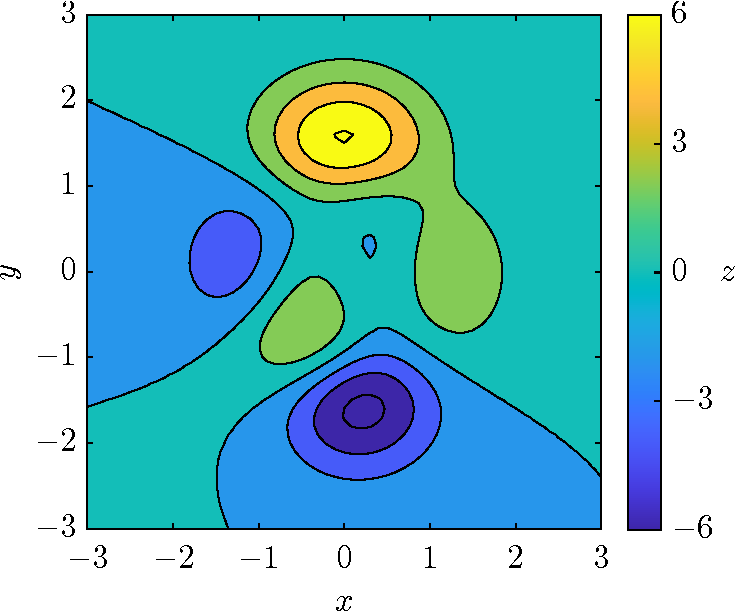
\includegraphics[width=\columnwidth]{figure/test1.pdf}
        \caption{PDF ファイル(文字抽出可).}
        \label{subfig:figcomp_pdf}
    \end{subfigure}
    \hfill % 水平方向のスペース
    \begin{subfigure}{0.45\columnwidth}
        \centering
        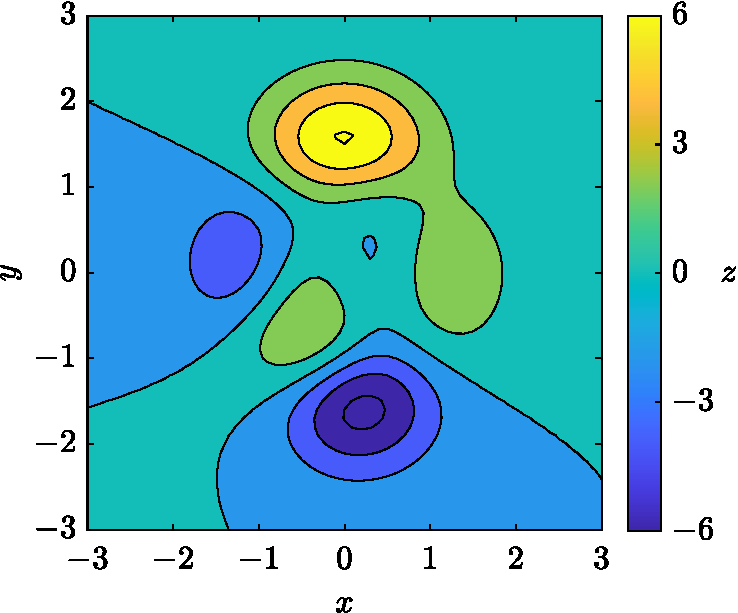
\includegraphics[width=\columnwidth]{figure/test2.pdf}
        \caption{PDF ファイル(文字抽出不可).}
        \label{subfig:figcomp_pdf2}
    \end{subfigure}

    \vspace{5mm} % 縦方向のスペース
    % 下の行
    \begin{subfigure}{0.45\columnwidth}
        \centering
        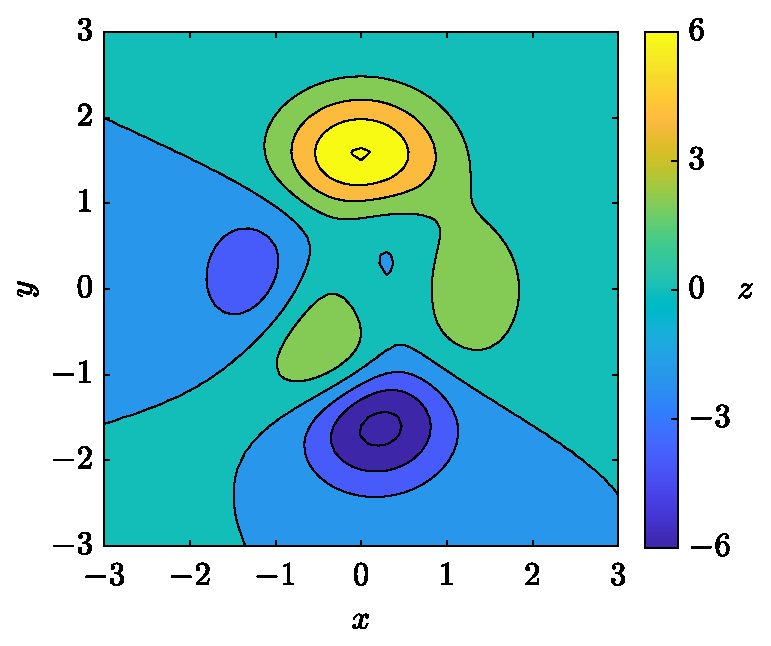
\includegraphics[width=\columnwidth]{figure/test3.eps}
        \caption{EPS ファイル.}
        \label{subfig:figcomp_eps}
    \end{subfigure}
    \hfill % 水平方向のスペース
    \begin{subfigure}{0.45\columnwidth}
        \centering
        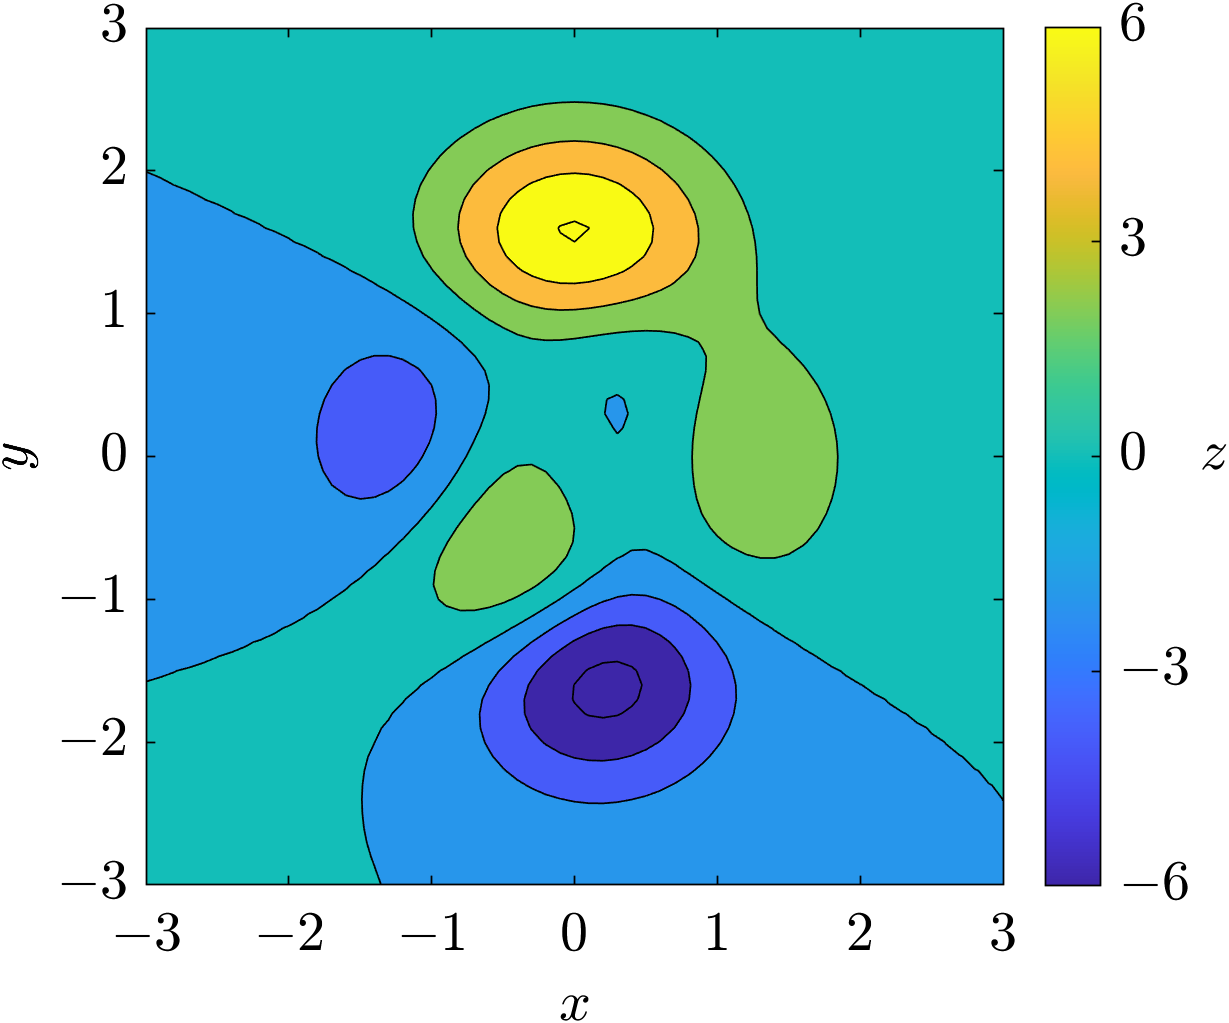
\includegraphics[width=\columnwidth]{figure/test4.png}
        \caption{PNG ファイル.}
        \label{subfig:figcomp_png}
    \end{subfigure}
    \caption{画像形式ごとの比較.}
    \label{fig:figure_comparison1}
\end{figure}

それでは実際にいくつかの画像形式を比較してみましょう.
図~\ref{fig:figure_comparison1} では (\subref{subfig:figcomp_pdf}, \subref{subfig:figcomp_pdf2}) PDF ファイル,(\subref{subfig:figcomp_eps}) EPS ファイル,(\subref{subfig:figcomp_png}) PNG ファイルを並べて比較しています.
パネル (\subref{subfig:figcomp_pdf}--\subref{subfig:figcomp_eps}) はどれもベクター画像なのでいくら拡大しても明瞭なままですね.
一方のパネル (\subref{subfig:figcomp_png}) を拡大するとラスター画像なので小さな正方形で構成されていることが確認できます.
これがベクター画像とラスター画像の違いです.
それではパネル (\subref{subfig:figcomp_pdf}) と (\subref{subfig:figcomp_pdf2}) の違いは何でしょうか.
どちらも PDF 形式ですよね.
\verb|main.pdf| を開きながら \verb|Ctrl|+\verb|A| をしてください.
パネル (\subref{subfig:figcomp_pdf}) は文字を抽出できますが,(\subref{subfig:figcomp_pdf2}) は文字を抽出できません.
皆さんが論文を書く際は (\subref{subfig:figcomp_pdf}) 文字抽出が可能な PDF を使用するのが理想です.


\section{表の配置}
\label{sec:table}






